% Single-column laboratory report template
% Adapted from original laboratory report layouts by Karol Cieślik (2017–2018).
% The sample content and numerical values below are fictional.
% Compile with pdfLaTeX + BibTeX, or use latexmk -pdf.

\documentclass[11pt,a4paper]{article}

\usepackage[T1]{fontenc}
\usepackage[utf8]{inputenc}
\usepackage[english]{babel}
\usepackage{lmodern}
\usepackage[margin=2.5cm]{geometry}
\usepackage{microtype}
\usepackage{amsmath}
\usepackage{booktabs}
\usepackage{graphicx}
\usepackage{pgfplots}
\usepackage{natbib}
\usepackage{fancyhdr}
\usepackage[hidelinks]{hyperref}

\pgfplotsset{compat=1.18}
\setlength{\parindent}{0.4cm}
\setlength{\parskip}{0.15em}
\setlength{\headheight}{15pt}
\emergencystretch=1em

% -------------------- Edit these fields --------------------
\newcommand{\reporttitle}{Electrical Characterisation of a Resistor}
\newcommand{\reportshorttitle}{Laboratory Report}
\newcommand{\reportauthor}{Student Name}
\newcommand{\reportinstitution}{Institution or Laboratory Name}
\newcommand{\reportcourse}{Course or Research Group}
\newcommand{\reportdate}{\today}
% -----------------------------------------------------------

\pagestyle{fancy}
\fancyhf{}
\fancyhead[L]{\small\scshape\reportshorttitle}
\fancyhead[R]{\small\scshape\reportauthor}
\fancyfoot[R]{\thepage}
\renewcommand{\headrulewidth}{0.4pt}

\begin{document}
% Avoid duplicate PDF page destinations when the page counter restarts
% after the unnumbered title page.
\hypersetup{pageanchor=false}
\begin{titlepage}
  \centering
  \vspace*{2.2cm}
  {\Large\scshape\reportinstitution\par}
  \vspace{0.6cm}
  {\large\reportcourse\par}
  \vspace{2cm}
  \rule{\textwidth}{0.5pt}\par
  \vspace{0.5cm}
  {\Huge\bfseries\reporttitle\par}
  \vspace{0.5cm}
  \rule{\textwidth}{1.7pt}\par
  \vspace{1.1cm}
  {\Large Laboratory Report\par}
  \vfill
  {\large\textbf{Author:} \reportauthor\par}
  \vspace{0.5cm}
  {\large\reportdate\par}
\end{titlepage}
\hypersetup{pageanchor=true}

\section*{Abstract}
This short example demonstrates how to format a scientific laboratory report.
A simple resistor is used as a familiar illustrative system. All values,
observations and uncertainties are \textbf{synthetic} and do not describe an
actual experiment. Replace this paragraph with the purpose, methods, central
findings and conclusion of your own work.

\section{Introduction}
\label{sec:introduction}
A laboratory report should explain the scientific question before presenting
measurements. For an ideal ohmic resistor, voltage \(V\) and current \(I\)
are related by
\begin{equation}
    V = IR,
    \label{eq:ohm}
\end{equation}
where \(R\) is the electrical resistance. Equation~\eqref{eq:ohm} is used
only to illustrate mathematical typesetting and cross-references.

\section{Experimental Methods}
\label{sec:methods}
Describe the instruments, sample preparation and measurement sequence in enough
detail to reproduce the work. Here, imagine a variable voltage source and a
current meter connected to a nominal \(1\,\mathrm{k}\Omega\) resistor.
Assume example standard uncertainties of \(0.01\,\mathrm{V}\) and
\(0.03\,\mathrm{mA}\), respectively. These are arbitrary teaching values.

Use consistent units and explain how uncertainties are estimated. A standard
introduction to uncertainty analysis is given by \citet{taylor1997}.

\section{Results}
\label{sec:results}
Table~\ref{tab:data} contains fictional observations. Numbers in an actual
report should be reported with sensible significant figures and should be
supported by the original measurement records.

\begin{table}[htbp]
    \centering
    \caption{Synthetic voltage-current values, for layout demonstration only.}
    \label{tab:data}
    \begin{tabular}{@{}rrr@{}}
        \toprule
        Voltage \(V\) (\(\mathrm{V}\)) &
        Current \(I\) (\(\mathrm{mA}\)) &
        Uncertainty \(u(I)\) (\(\mathrm{mA}\)) \\
        \midrule
        0.50 & 0.50 & 0.03 \\
        1.00 & 1.01 & 0.03 \\
        1.50 & 1.49 & 0.03 \\
        2.00 & 2.02 & 0.03 \\
        2.50 & 2.49 & 0.03 \\
        3.00 & 3.01 & 0.03 \\
        \bottomrule
    \end{tabular}
\end{table}

Figure~\ref{fig:current-voltage} illustrates a compact plot generated directly
in LaTeX. The solid line is an ideal reference curve, not a fit to real data.

\clearpage
\begin{figure}[htbp]
    \centering
    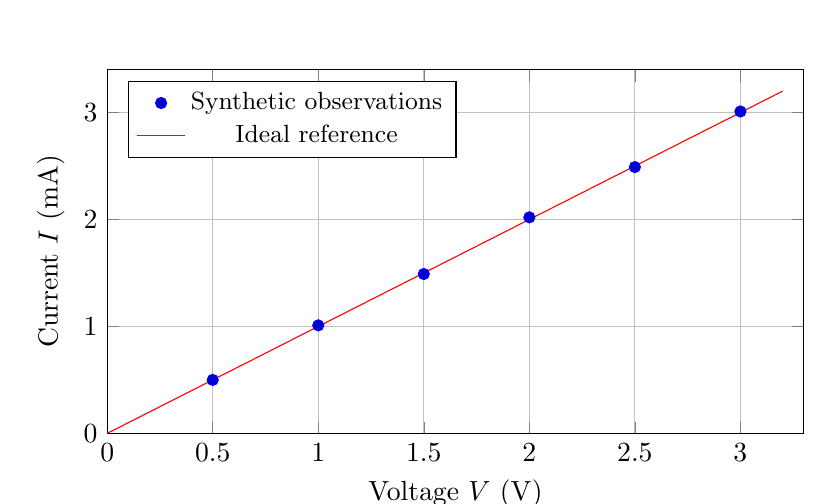
\begin{tikzpicture}
        \begin{axis}[
            width=0.86\linewidth,
            height=6.2cm,
            xlabel={Voltage \(V\) (\(\mathrm{V}\))},
            ylabel={Current \(I\) (\(\mathrm{mA}\))},
            xmin=0, xmax=3.3,
            ymin=0, ymax=3.4,
            grid=major,
            legend pos=north west,
            legend style={font=\small},
        ]
            \addplot+[only marks, mark=*] coordinates {
                (0.50,0.50) (1.00,1.01) (1.50,1.49)
                (2.00,2.02) (2.50,2.49) (3.00,3.01)
            };
            \addlegendentry{Synthetic observations}
            \addplot+[no marks, domain=0:3.2, samples=2] {x};
            \addlegendentry{Ideal reference}
        \end{axis}
    \end{tikzpicture}
    \caption{Illustrative current-voltage relationship. The data are synthetic.}
    \label{fig:current-voltage}
\end{figure}

\section{Discussion}
\label{sec:discussion}
Discuss the physical interpretation rather than simply restating the results.
For example, a resistance could be calculated from the slope of current
against voltage. Under an independence assumption, illustrative propagation
for \(R=V/I\) is
\begin{equation}
    \frac{u(R)}{R}
    \approx
    \sqrt{\left(\frac{u(V)}{V}\right)^2+
          \left(\frac{u(I)}{I}\right)^2}.
    \label{eq:uncertainty}
\end{equation}
Explain whether the assumptions behind Equation~\eqref{eq:uncertainty} are
appropriate for the real experiment and distinguish random from systematic
effects.

\section{Conclusion}
State what was established, what remains uncertain and what might improve a
future measurement. Delete all fictional example content when adapting this
template for an actual laboratory report.

\bibliographystyle{unsrtnat}
\bibliography{references}

\end{document}
